\documentclass[6pt]{article}
\usepackage[margin=0.3in, landscape, letterpaper]{geometry}
\usepackage{amsmath, amssymb}
\usepackage{enumitem}
\usepackage{booktabs}
\usepackage{xcolor}
\usepackage{multicol}
\usepackage{float}
\usepackage{tikz}
\usepackage{tcolorbox}
\usepackage{titlesec}
\usetikzlibrary{arrows.meta, positioning, calc}

% Brand colors
\definecolor{garnet}{HTML}{73000A}
\definecolor{black90}{HTML}{363636}
\definecolor{black70}{HTML}{5C5C5C}
\definecolor{atlantic}{HTML}{466A9F}
\definecolor{congaree}{HTML}{1F414D}
\definecolor{horseshoe}{HTML}{65780B}
\definecolor{rose}{HTML}{CC2E40}
\definecolor{honeycomb}{HTML}{A49137}
\definecolor{grass}{HTML}{CED318}
\definecolor{sandstorm}{HTML}{FFF2E3}
\definecolor{black10}{HTML}{ECECEC}

\color{black90}

% Compact spacing
\setlength{\parskip}{1pt}
\setlength{\parindent}{0pt}
\setlength{\columnsep}{8pt}
\setlength{\columnseprule}{0.4pt}
\def\columnseprulecolor{\color{black!20}}

% Compact sections
\titleformat{\section}{\normalsize\bfseries\color{garnet}}{}{0pt}{}
\titlespacing*{\section}{0pt}{4pt}{1pt}
\titleformat{\subsection}{\small\bfseries\color{atlantic}}{}{0pt}{}
\titlespacing*{\subsection}{0pt}{3pt}{0.5pt}

% Colored boxes
\tcbset{
    boxrule=0.5pt,
    arc=0pt, outer arc=0pt,
    left=2pt, right=2pt, top=1pt, bottom=1pt,
    fontupper=\scriptsize,
}

\newcommand{\mathbox}[2]{%
\begin{tcolorbox}[colback=sandstorm, colframe=garnet, title={\scriptsize\bfseries\color{white}#1}, coltitle=white, colbacktitle=garnet, toptitle=1pt, bottomtitle=1pt]
#2
\end{tcolorbox}
}

\newcommand{\conceptbox}[2]{%
\begin{tcolorbox}[colback=atlantic!5, colframe=atlantic, title={\scriptsize\bfseries\color{white}#1}, coltitle=white, colbacktitle=atlantic, toptitle=1pt, bottomtitle=1pt]
#2
\end{tcolorbox}
}

\newcommand{\warnbox}[1]{%
\begin{tcolorbox}[colback=rose!8, colframe=rose, boxrule=0.8pt]
\textcolor{rose}{\textbf{!}} #1
\end{tcolorbox}
}

\pagestyle{empty}

\begin{document}

% ====================== PAGE 1: CONCEPTS ======================
\begin{center}
{\large\bfseries\color{garnet} CSCE 775 Quiz 2 Cheat Sheet --- Page 1: Concepts}\quad{\scriptsize\color{black70} Lectures 4--7}
\end{center}
\vspace{-4pt}
\hrule height 1pt
\vspace{2pt}

\begin{multicols}{4}

\section{Model-Free RL}

\conceptbox{MC vs TD vs $n$-step}{
\begin{tabular}{@{}lccc@{}}
& \textbf{MC} & \textbf{TD} & $n$\textbf{-step} \\
\midrule
Target & $G_t$ & $R\!+\!\gamma V(S')$ & mixed \\
Bias & None & Yes & Med \\
Var & High & Low & Med \\
Episodes? & Must end & Online & Online \\
Bootstrap? & No & Yes & Yes \\
\end{tabular}
}

\subsection{On-Policy vs Off-Policy}
\textbf{Behavior} $b$: collects data\\
\textbf{Target} $\pi$: being improved\\
\textbf{On:} $b = \pi$ (SARSA, MC)\\
\textbf{Off:} $b \neq \pi$ (Q-learning)

\subsection{$\varepsilon$-Greedy}
Greedy: $1 - \varepsilon + \varepsilon/|\mathcal{A}|$\\
Other: $\varepsilon/|\mathcal{A}|$ each\\
\textit{Why?} Pure greedy gets stuck.

\subsection{SARSA vs Q-Learning}

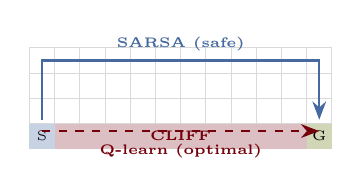
\begin{tikzpicture}[scale=0.32, every node/.style={font=\tiny}]
    \foreach \x in {0,...,11} \foreach \y in {0,...,3}
        \draw[black!15] (\x,\y) rectangle (\x+1,\y+1);
    \foreach \x in {1,...,10}
        \fill[garnet!25] (\x,0) rectangle (\x+1,1);
    \node[garnet, font=\tiny\bfseries] at (6, 0.5) {CLIFF};
    \fill[atlantic!30] (0,0) rectangle (1,1);
    \node at (0.5,0.5) {S};
    \fill[horseshoe!30] (11,0) rectangle (12,1);
    \node at (11.5,0.5) {G};
    \draw[-{Stealth}, atlantic, thick] (0.5,1.15) -- (0.5,3.5) -- (11.5,3.5) -- (11.5,1.15);
    \node[atlantic, above, font=\tiny\bfseries] at (6,3.5) {SARSA (safe)};
    \draw[-{Stealth}, garnet, thick, dashed] (0.5,0.7) -- (11.5,0.7);
    \node[garnet, below, font=\tiny\bfseries] at (6,0.55) {Q-learn (optimal)};
\end{tikzpicture}

SARSA: cautious (on-policy)\\
Q-learn: optimal (off-policy)

\subsection{Bootstrapping}
Using estimates to update estimates.\\
TD: yes (biased, fast). MC: no (unbiased, slow).

\subsection{$n$-Step \& TD($\lambda$)}
$n\!=\!1$: TD(0). $n\!=\!\infty$: MC. Best $\approx 5$.\\
TD($\lambda$): weighted avg of all $n$-step.\\
$\lambda\!=\!0$: TD(0). $\lambda\!=\!1$: MC.

\subsection{Why $Q$ not $V$?}
No model $\Rightarrow$ can't derive $\pi$ from $V$.\\
$Q$: just take $\arg\max_a Q(s,a)$.

\vfill\null
\columnbreak

% ---- COLUMN 2: DEEP LEARNING ----
\section{Deep Learning}

\conceptbox{Neural Networks}{
$f(\mathbf{x}) = \mathbf{W}^{(2)}\sigma(\mathbf{W}^{(1)}\mathbf{x} + \mathbf{b}^{(1)}) + \mathbf{b}^{(2)}$

\textbf{Non-linear activations required!}\\
Without: $\mathbf{W}_2\mathbf{W}_1\mathbf{x} = \mathbf{W}'\mathbf{x}$ (linear)
}

\subsection{Activations}
\textbf{Sigmoid:} $\frac{1}{1+e^{-x}}$, out $(0,1)$, vanish grad\\
\textbf{Tanh:} out $(-1,1)$\\
\textbf{ReLU:} $\max(0,x)$ --- most common\\
\textbf{Leaky ReLU:} $\max(0.01x,x)$

\subsection{Overfitting Fixes}
Regularization ($\lambda\!\sum\! W^2$), dropout,
data augmentation, early stopping

\subsection{Optimizers}
\textbf{SGD:} $\mathbf{w} \leftarrow \mathbf{w} - \alpha\nabla E$\\
\textbf{Momentum:} accumulate velocity\\
$\mathbf{v} \leftarrow \mu\mathbf{v} + \alpha\nabla E$;\ $\mathbf{w} \leftarrow \mathbf{w} - \mathbf{v}$\\
\textbf{ADAM:} adaptive lr per param

\subsection{ResNets \& BatchNorm}
\textbf{Skip:} out $= F(\mathbf{x}) + \mathbf{x}$\\
$\nabla$: $F' + \mathbf{I}$ ($\geq 1$, no vanishing!)\\
\textbf{BN:} normalize to $\mu\!=\!0,\sigma\!=\!1$

\subsection{Params vs Hyperparams}
\textbf{Params:} learned (weights, biases)\\
\textbf{Hyper:} set before (lr, layers, $\varepsilon$)

\subsection{Backpropagation}
Chain rule layer by layer.\\
\textbf{Pattern:} error $\times$ weight $\times$ $\sigma'$ $\times$ input\\
Errors flow backward through network.

\subsection{Universal Approx.\ Theorem}
Enough hidden units $\to$ approx \textit{any}
continuous function. Does NOT guarantee
training converges.

\vfill\null
\columnbreak

% ---- COLUMN 3: PYTORCH + DQN ----
\section{PyTorch}

\conceptbox{Training Loop (memorize!)}{
\texttt{1. optimizer.zero\_grad()}\\
\hspace*{1em}{\color{black70}\scriptsize clear old gradients}\\
\texttt{2. out = nnet(x)}\\
\hspace*{1em}{\color{black70}\scriptsize forward pass}\\
\texttt{3. loss = criterion(out, y)}\\
\texttt{4. loss.backward()}\\
\hspace*{1em}{\color{black70}\scriptsize compute $\nabla_\theta\mathcal{L}$}\\
\texttt{5. optimizer.step()}\\
\hspace*{1em}{\color{black70}\scriptsize $\theta \leftarrow \theta - \alpha\nabla$}
}

\vspace{2pt}
\texttt{.detach()} = stop gradient flow\\
\texttt{loss.item()} = scalar (no mem leak)\\
\texttt{.train()} = dropout ON\\
\texttt{.eval()} = dropout OFF\\
\texttt{torch.save(nnet.state\_dict())}\\
\hspace*{1em}= save params only

\subsection{Gradient Checking}
$\frac{\partial f}{\partial\theta_i} \approx \frac{f(\theta_i+h)-f(\theta_i)}{h}$,\ $h\!\approx\!10^{-5}$

\section{DQN}

\conceptbox{Three DQN Innovations}{
\textbf{1. Target network} $\theta^-$:\\
\hspace*{1em}freeze target for $C$ steps\\
\textbf{2. Experience replay}:\\
\hspace*{1em}store $(s,a,r,s')$, sample random\\
\hspace*{1em}batches (breaks correlation)\\
\textbf{3. Huber loss}:\\
\hspace*{1em}clips grads for large TD errors
}

\vspace{2pt}
\warnbox{Removing \textit{either} replay OR target net $\to$ catastrophic failure}

\subsection{DQN Improvements}
\textbf{Double Q:} one net picks action,\\
\hspace*{1em}other evaluates (fix max bias)\\
\textbf{Dueling:} $q = v(s) + A(s,a)$\\
\hspace*{1em}separate state \& action value\\
\textbf{Prioritized replay:} sample\\
\hspace*{1em}large-error transitions more\\
\textbf{Rainbow:} all combined\\
\textbf{Agent57:} beats all 57 Atari

\vfill\null
\columnbreak

% ---- COLUMN 4: KEY EQUATIONS ----
\section{Key Equations}

\conceptbox{Update Rules}{
\textbf{MC:}\\
$V(S_t) \!\leftarrow\! V(S_t) + \alpha(G_t - V(S_t))$

\vspace{2pt}
\textbf{TD(0):}\\
$V(S_t) \!\leftarrow\! V(S_t) + \alpha[\underbrace{R\!+\!\gamma V(S')}_{\text{target}}\!-\!V(S_t)]$

\vspace{2pt}
\textbf{SARSA} (on-policy):\\
$Q(S,\!A) \!\leftarrow\! Q(S,\!A)$\\
$\;+\alpha[R\!+\!\gamma Q(S'\!,\textcolor{atlantic}{A'})\!-\!Q(S,\!A)]$

\vspace{2pt}
\textbf{Q-learn} (off-policy):\\
$Q(S,\!A) \!\leftarrow\! Q(S,\!A)$\\
$\;+\alpha[R\!+\!\gamma\textcolor{garnet}{\max_a}Q(S'\!,a)\!-\!Q(S,\!A)]$

\vspace{2pt}
\textbf{DQN Target:}\\
$y = R + \gamma\max_{a'}q_{\textcolor{rose}{\theta^-}}(S',a')$\\
$L = \frac{1}{2}(y - q_\theta(S,A))^2$

\vspace{2pt}
\textbf{$n$-step return:}\\
$G_{t:t+n} = \sum_{k=0}^{n-1}\gamma^k R_{t\!+\!k\!+\!1} + \gamma^n V(S_{t+n})$
}

\vspace{3pt}

\conceptbox{Important Definitions}{
\textbf{TD error:}\\
$\delta_t = R_{t+1} + \gamma V(S_{t+1}) - V(S_t)$

\vspace{2pt}
\textbf{Advantage:}\\
$A_\pi(s,a) = q_\pi(s,a) - v_\pi(s)$

\vspace{2pt}
\textbf{Sigmoid:}\\
$\sigma(z) = \frac{1}{1+e^{-z}}$,\quad $\sigma' = \sigma(1\!-\!\sigma)$

\vspace{2pt}
\textbf{Softmax:}\\
$P(y\!=\!i|\mathbf{x}) = \frac{e^{\mathbf{w}_i^\top\mathbf{x}}}{\sum_j e^{\mathbf{w}_j^\top\mathbf{x}}}$

\vspace{2pt}
\textbf{Cross-entropy loss:}\\
$\mathcal{L} = -\!\sum_i[y_i\log\hat{y}_i + (1\!-\!y_i)\log(1\!-\!\hat{y}_i)]$

\vspace{2pt}
\textbf{Robbins-Monro:}\\
$\sum\alpha_n = \infty$,\quad $\sum\alpha_n^2 < \infty$
}

\end{multicols}

% ====================== PAGE 2: MATH ======================
\newpage

\begin{center}
{\large\bfseries\color{garnet} CSCE 775 Quiz 2 Cheat Sheet --- Page 2: Derivations}\quad{\scriptsize\color{black70} All 7 likely derivation problems}
\end{center}
\vspace{-4pt}
\hrule height 1pt
\vspace{2pt}

\begin{multicols}{4}

\mathbox{1. MC Incremental Update}{
\textit{Show running average = incremental form.}

Start: $V_n = \frac{1}{n}\sum_{k=1}^n G_k$

Split off $n$-th term:
\begin{align*}
V_n &= \frac{1}{n}\Bigl(G_n + (n\!-\!1)V_{n-1}\Bigr)\\
&= \frac{1}{n}G_n + \frac{n\!-\!1}{n}V_{n-1}\\
&= \frac{1}{n}G_n + V_{n-1} - \frac{1}{n}V_{n-1}\\
&= V_{n-1} + \frac{1}{n}\bigl(G_n - V_{n-1}\bigr)
\end{align*}
\[\boxed{V(S_t) \leftarrow V(S_t) + \alpha\bigl(G_t - V(S_t)\bigr)}\]
\textbf{Trick:} $\frac{n-1}{n} = 1 - \frac{1}{n}$
}

\vspace{3pt}

\mathbox{2. $\varepsilon$-Greedy Improvement}{
\textit{Show $q_\pi(s,\pi'(s)) \geq v_\pi(s)$.}
\begin{align*}
&\sum_a \pi'(a|s)\,q_\pi(s,a) \\
&= \frac{\varepsilon}{|\mathcal{A}|}\sum_a q_\pi(s,a)\\
&\quad + (1\!-\!\varepsilon)\max_a q_\pi(s,a)
\end{align*}
Since $\max \geq$ weighted avg, use weights
$w_a = \frac{\pi(a|s) - \varepsilon/|\mathcal{A}|}{1-\varepsilon}$:
\begin{align*}
&\geq \frac{\varepsilon}{|\mathcal{A}|}\sum_a q_\pi\\
&\quad + \sum_a\bigl(\pi(a|s) - \tfrac{\varepsilon}{|\mathcal{A}|}\bigr)q_\pi\\
&= \sum_a \pi(a|s)\,q_\pi(s,a)\\
&= v_\pi(s) \quad\square
\end{align*}
By policy improvement theorem:\\
$v_{\pi'}(s) \geq v_\pi(s)\ \forall s$.
}

\vfill\null
\columnbreak

\mathbox{3. Sigmoid Derivative}{
\textit{Derive $\frac{d}{dz}\sigma(z)$.}

$\sigma(z) = (1+e^{-z})^{-1}$

Apply chain rule:
\begin{align*}
\sigma' &= -(1+e^{-z})^{-2}\cdot(-e^{-z})\\
&= \frac{e^{-z}}{(1+e^{-z})^2}
\end{align*}

Factor:
\begin{align*}
&= \frac{1}{1\!+\!e^{-z}}\cdot\frac{e^{-z}}{1\!+\!e^{-z}}\\
&= \sigma\cdot\frac{(1\!+\!e^{-z})-1}{1\!+\!e^{-z}}\\
&= \sigma\cdot(1-\sigma)
\end{align*}

\[\boxed{\sigma'(z) = \sigma(z)(1-\sigma(z))}\]

Max at $z\!=\!0$: $\sigma'\!=\!0.25$\\
$\to$ vanishing gradients in deep nets
}

\vspace{3pt}

\mathbox{4. Logistic Regression Gradient}{
\textit{Derive $\nabla_\mathbf{w}\mathcal{L}$ for cross-entropy.}

One sample: $\hat{y}=\sigma(\mathbf{w}^\top\mathbf{x})$
\[
\ell = y\log\hat{y} + (1\!-\!y)\log(1\!-\!\hat{y})
\]

Using $\sigma' = \sigma(1\!-\!\sigma)$:
\begin{align*}
\frac{\partial\ell}{\partial\mathbf{w}} &= y\frac{\sigma(1\!-\!\sigma)}{\sigma}\mathbf{x} + (1\!-\!y)\frac{-\sigma(1\!-\!\sigma)}{1\!-\!\sigma}\mathbf{x}\\
&= y(1\!-\!\hat{y})\mathbf{x} - (1\!-\!y)\hat{y}\,\mathbf{x}\\
&= (y - \hat{y})\,\mathbf{x}
\end{align*}

Loss $= -\ell$, so over $N$ samples:
\[\boxed{\nabla_\mathbf{w}\mathcal{L} = \frac{1}{N}\sum_{i}(\hat{y}_i - y_i)\mathbf{x}_i}\]

\textbf{Key:} $\sigma'$ cancels the denominators!
}

\vfill\null
\columnbreak

\mathbox{5. Backprop (2-Layer Net)}{
\textit{Derive weight gradients.}

$\hat{\mathbf{y}} = \mathbf{W}^{(2)}\mathbf{h}$,\quad $\mathbf{h} = \sigma(\mathbf{W}^{(1)}\mathbf{x})$

$E = \frac{1}{2}\sum_i(y_i - \hat{y}_i)^2$

\textbf{Output layer} (one chain rule):
\begin{align*}
\frac{\partial E}{\partial W_{ij}^{(2)}} &= \frac{\partial E}{\partial\hat{y}_i}\cdot\frac{\partial\hat{y}_i}{\partial W_{ij}^{(2)}}\\
&= -(y_i - \hat{y}_i)\cdot h_j
\end{align*}

\textbf{Hidden layer} (two chain rules):
\begin{align*}
\frac{\partial E}{\partial W_{jk}^{(1)}} &= \sum_i\frac{\partial E}{\partial\hat{y}_i}\cdot\frac{\partial\hat{y}_i}{\partial h_j}\cdot\frac{\partial h_j}{\partial W_{jk}^{(1)}}\\
&= \underbrace{\sum_i[-(y_i\!-\!\hat{y}_i)]W_{ij}^{(2)}}_{\text{backprop error}}\\
&\quad\cdot\;\sigma'(\mathbf{W}^{(1)}_j\mathbf{x})\cdot x_k
\end{align*}

\textbf{Pattern:}\\
error $\times$ weight $\times$ $\sigma'$ $\times$ input
}

\vspace{3pt}

\mathbox{6. DAVI Gradient}{
\textit{Derive the gradient of AVI loss.}

Target {\color{rose}(treat as constant!)}:
\[
y = \max_a\!\Bigl[r(s,a) + \gamma\!\sum_{s'}p(s'|s,a)v_{\theta^-}(s')\Bigr]
\]

Loss: $L(\theta) = \frac{1}{2}(y - v_\theta(s))^2$

Do NOT differentiate $y$:
\begin{align*}
\nabla_\theta L &= (y\!-\!v_\theta(s))(-\nabla_\theta v_\theta(s))
\end{align*}

Update rule:
\[\boxed{\theta \leftarrow \theta + \alpha(y\!-\!v_\theta(s))\nabla_\theta v_\theta(s)}\]

$y$ uses $\theta^-$ (frozen target net).\\
PyTorch: \texttt{.detach()} or \texttt{no\_grad()}
}

\vfill\null
\columnbreak

\mathbox{7. Linear Regression Closed Form}{
\textit{Derive $\mathbf{w}^*$ analytically.}

$\hat{\mathbf{y}} = \mathbf{X}\mathbf{w}$

$\mathcal{L} = (\mathbf{X}\mathbf{w}\!-\!\mathbf{y})^\top(\mathbf{X}\mathbf{w}\!-\!\mathbf{y})$

Expand:
\begin{align*}
\mathcal{L} &= \mathbf{w}^\top\mathbf{X}^\top\mathbf{X}\mathbf{w} - 2\mathbf{w}^\top\mathbf{X}^\top\mathbf{y} + \mathbf{y}^\top\mathbf{y}
\end{align*}

Set gradient to zero:
\begin{align*}
\nabla_\mathbf{w}\mathcal{L} &= 2\mathbf{X}^\top\mathbf{X}\mathbf{w} - 2\mathbf{X}^\top\mathbf{y} = \mathbf{0}
\end{align*}

Solve:
\[\boxed{\mathbf{w}^* = (\mathbf{X}^\top\mathbf{X})^{-1}\mathbf{X}^\top\mathbf{y}}\]

Key: $\nabla_\mathbf{w}(\mathbf{w}^\top\!\mathbf{A}\mathbf{w}) = 2\mathbf{A}\mathbf{w}$
}

\vspace{4pt}

\warnbox{\textbf{Derivation Tricks:}\\[1pt]
$\bullet$ Split last term: $\sum_1^n = \sum_1^{n-1} + n$th\\
$\bullet$ $\sigma'\!=\!\sigma(1\!-\!\sigma)$ cancels log denoms\\
$\bullet$ $\max f \geq \sum w_a f$ (convex wts)\\
$\bullet$ Chain rule = multiply $\nabla$ per layer\\
$\bullet$ $\nabla_\mathbf{w}(\mathbf{w}^\top\!\mathbf{A}\mathbf{w}) = 2\mathbf{A}\mathbf{w}$\\
$\bullet$ \textbf{Never} diff target $y$ in DAVI/DQN
}

\vspace{4pt}

\conceptbox{DAVI vs DQN}{
\textbf{DAVI:} knows model $p(s'|s,a)$\\
$y = \max_a[r + \gamma\sum_{s'}p\cdot v_{\theta^-}]$\\
Approximates $v_*(s)$

\vspace{2pt}
\textbf{DQN:} model-free\\
$y = r + \gamma\max_{a'}q_{\theta^-}(s',a')$\\
Approximates $q_*(s,a)$

\vspace{2pt}
Both use target networks.\\
DQN also needs replay buffer.
}

\end{multicols}

\end{document}
